\documentclass[12pt]{article}
\usepackage{graphicx,amsthm,amsmath,amssymb,algorithm,algorithmic,geometry,setspace,fancyhdr,varwidth,subfig,pdfpages,float}
\usepackage[english]{babel}
\usepackage[colorlinks=true,linkcolor=blue]{hyperref}
\usepackage[superscript,biblabel]{cite}
\usepackage[export]{adjustbox}
\geometry{letterpaper,
	total={170mm,257mm},
	left=20mm,
	top=30mm, bottom=20mm}  % or letter or a5paper or ... etc
% \geometry{landscape} % rotated page geometry

\title{Ph 20: Assignment \#2}
\author{Maya Fuller}
\date{Due: April 16, 2018} % delete this line to display the current date

% See the ``Article customise'' template for come common customisation

\begin{document}
	
	\pagenumbering{gobble}
	
	\maketitle

	\noindent\textbf{\large Problem 1}\\[5mm]
		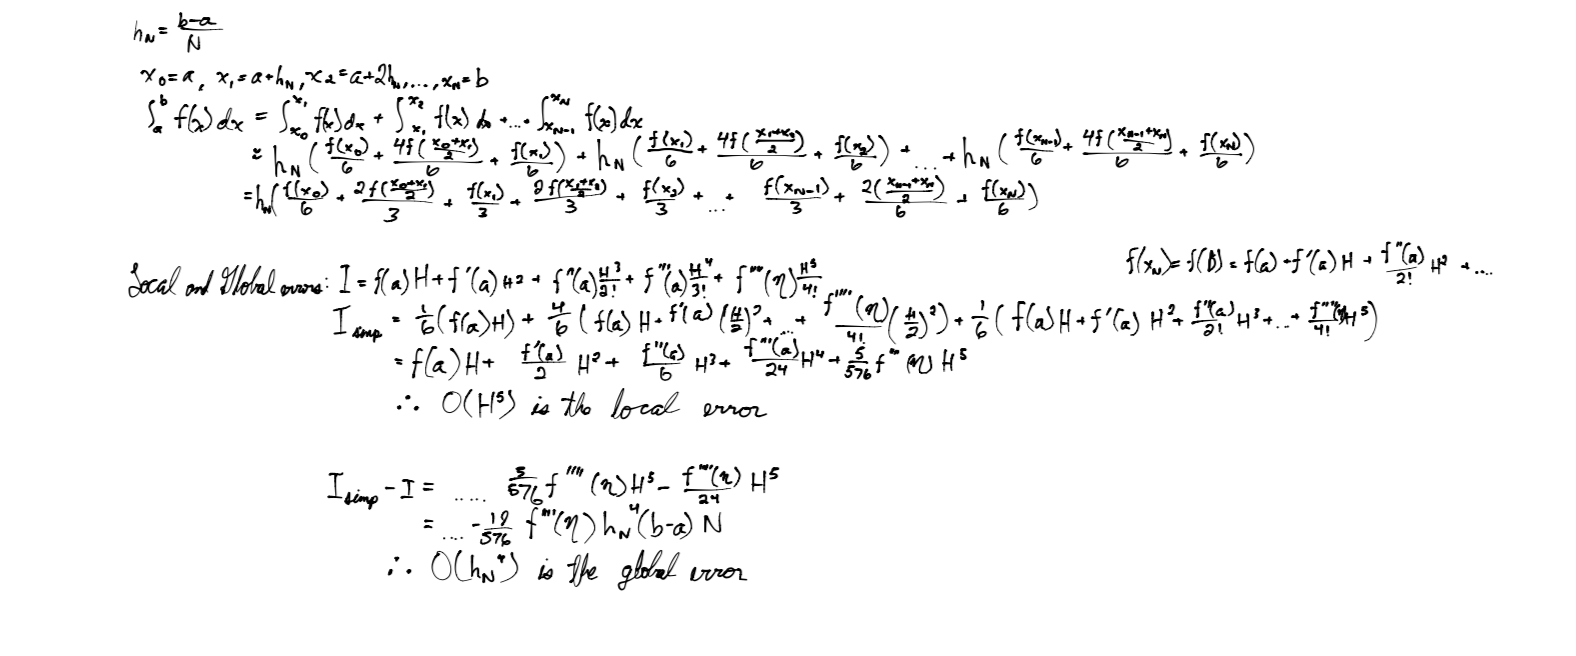
\includegraphics[width=\textwidth]{derivation.png}
	
	\noindent\textbf{\large Problem 2}\\
		See Python file\\[5mm]
	\noindent\textbf{\large Problem 3}\\
		See Python file \\[5mm]
	\noindent\textbf{\large Problem 4}
		\begin{center}
				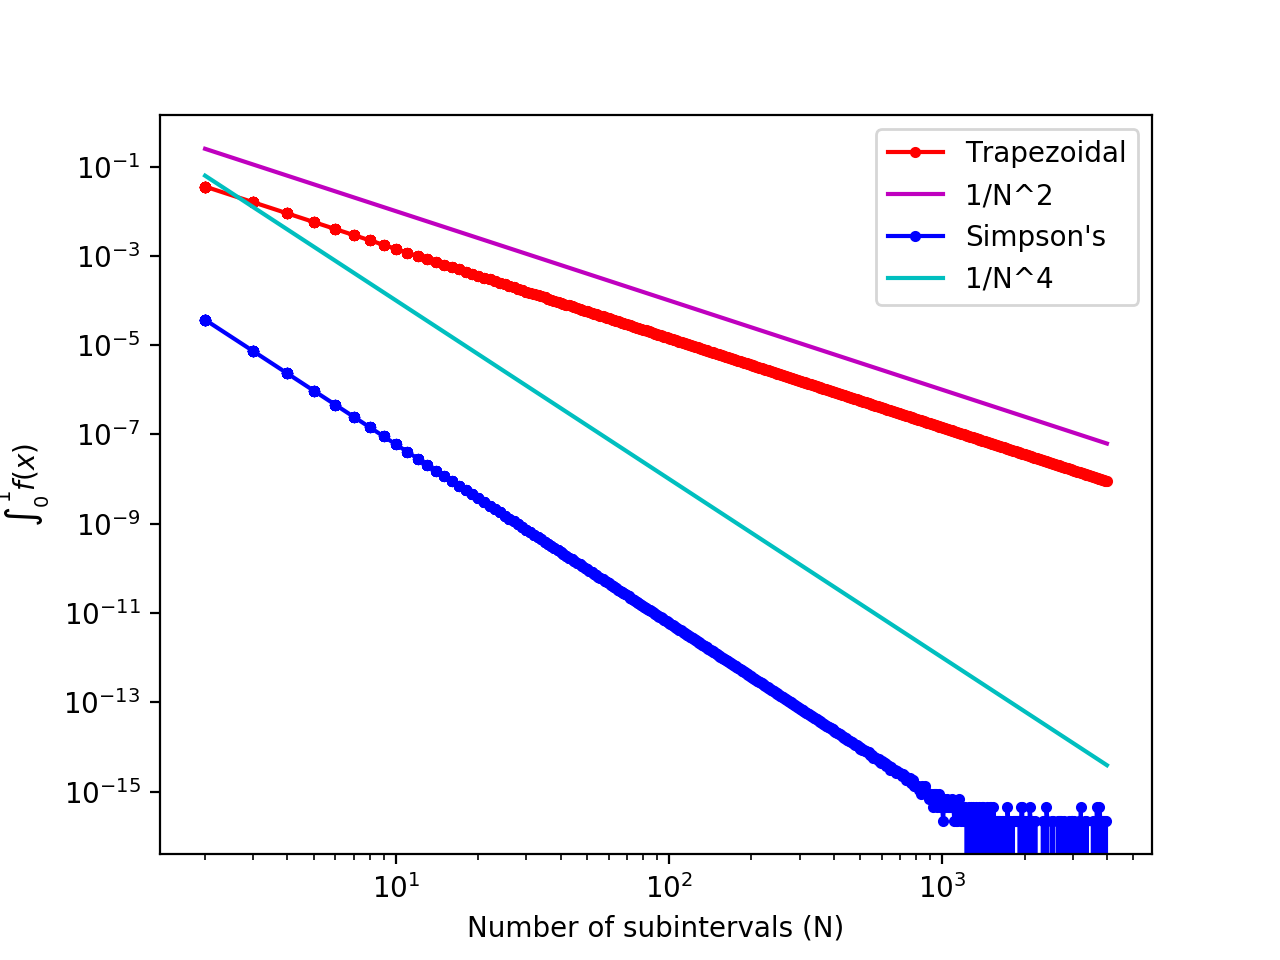
\includegraphics[width=0.8\textwidth]{prob4.png}
		\end{center}		
		See Python file\\[5mm]
	\noindent\textbf{\large Problem 6}\\
		See Python file\\[5mm]
	\noindent\textbf{\large Problem 7}\\
		See Python file
			
		
\end{document}